%----------------------------------------------------------------------------
\section{Some math(s)}
%----------------------------------------------------------------------------

\begin{frame}

\begin{center}
{\LARGE Appendix: Some math(s)}
\end{center}

\end{frame}

%----------------------------------------------------------------------------

%----------------------------------------------------------------------------

\begin{frame}{Unofficial maths `requirements'}

Most of the maths we use will entail\ldots
\begin{itemize}
\item	Basic algebra
	\begin{itemize}
	\item	$C_{t}$ will represent consumption in time $t$
	\end{itemize}
\item	Basic probability
	\begin{itemize}
	\item	Mean/expectation and maybe standard deviation
	\end{itemize}
\item	Collecting coefficients / factorization
	\begin{itemize}
	\item	$a x + bx = (a+b)x$
	\end{itemize}
\item	Summations
	\begin{itemize}
	\item	$\sum\limits_{j=0}^{J} f(x_{j}) \equiv f(x_{0})+f(x_{1}) +\ldots+f(x_{J})$
	\end{itemize}
\item	Calculus
	\begin{itemize}
	\item	You will need to differentiate very simple functions
	\item	You will probably only need to understand what an integral ($\int$) \emph{means}
	\item	\textcolor{red}{You will need to be able to linearize and log-linearize}
	\end{itemize}
\end{itemize}

\end{frame}

%-------------------------------------------------------

%-------------------------------------------------------

\begin{frame}{Solving an economic model}

What does it mean to `solve' an economic model?
\begin{itemize}
\item	Models involve a lot of `variables' (consumption, unemployment, output, wages,\ldots)
\item	Accounting and technological constraints imply relationships among these variables
\item	The assumption that people and firms are optimizing also implies relationships among these variables
\item	There is a core set of variables that are needed to describe `the current situation' (all the relevant info.)
\item	We call these variables `the state'
\item	\textbf{Solving a model $\Leftrightarrow$ finding functions that relate all the variables in the economy to the state}
\end{itemize}

\end{frame}

%-------------------------------------------------------

%-------------------------------------------------------

\begin{frame}{Taylor approximations}

Consider consumption in time $t$, $C_{t}$
\begin{itemize}
\item	A solved model implies
\[
C_{t} = f(tax\text{ }rate, income, assets, monetary\text{ }policy, \ldots)
\]
\item	Or let's just call the state, $s_{t}$
\[
C_{t} = f(s_{t})
\]
\item	Sadly, it is rare that the function $f$ can actually be calculated
\item	Happily, we can more often calculate its derivatives
\item	Remember Taylor approximations from high school - e.g. $2^{nd}$ order\ldots
\[
f(s_{t}) \approx f(\bar{s}) + f'(\bar{s})(s_{t}-\bar{s}) + \frac{1}{2!}f''(\bar{s})(s_{t}-\bar{s})^{2}
\]
\end{itemize}

\end{frame}

%-------------------------------------------------------

%-------------------------------------------------------

\begin{frame}{Taylor approximations}

In this course, we don't even need second order!
\begin{itemize}
\item	We will only work with first order approximations
\item	\textbf{In fact, at $1^{st}$ order we proceed simply by linearizing the equations describing technological constraints and firm/household optimality}
\item	If we solve those linear equations (like in high school) we will obtain a first order approximation to $f$
\item	For more info on `higher-order asymptotic approximations' and `perturbation methods' see\ldots
	\begin{itemize}
	\item \url{https://www.nber.org/econometrics_minicourse_2011/Chapter_2_Pertubation.pdf}
	\end{itemize}
\end{itemize}

\vspace{2mm}
So we need to be reminded how to take a linear approximation

\end{frame}

%-------------------------------------------------------

%-------------------------------------------------------

\begin{frame}{Linearization - scalar case}

Under various assumptions (that I won't describe here but which hold for the models we consider)
\[
f(x) \approx f(\bar{x}) + f'(\bar{x})(x-\bar{x})
\]
where
\[
f'(\bar{x}) \equiv \frac{df}{dx}(\bar{x})
\]

This is a first order approximation of $f$ with respect to $x$, around the point $x = \bar{x}$

\end{frame}

%-------------------------------------------------------

%-------------------------------------------------------

\begin{frame}{Linearization - scalar case}

A linear approximation will be exact if $f$ is linear to begin with
\begin{itemize}
\item	Consider $f(x) = \alpha x$
\item	$f'(x) = \alpha$ for all $x$
\item	$f(x) \stackrel{Exact}= f(\bar{x}) +  \alpha (x-\bar{x}) = \alpha x = f(x)$ for all $\bar{x}$
\item	Clearly, this is pointless
\end{itemize}

\vspace{2mm}
Consider a more general case of a quadratic $f$
\begin{itemize}
\item	Consider $f(x) = \frac{\alpha}{2} x^{2}$
\item	$f'(x) = \alpha x$
\item	$f(x) \approx f(\bar{x}) +  \alpha \bar{x} (x-\bar{x}) \equiv \hat{f}(x)$ for arbitrary $x$
\item	$f(x) \stackrel{Exact}= f(\bar{x}) +  \alpha \bar{x} (x-\bar{x}) = f(\bar{x})$ only for $x=\bar{x}$ (trivially)
\end{itemize}

\vspace{2mm}
We take a slope at a point and then using the linear function with \emph{that slope} from \emph{that point}, to approximate the function of interest \emph{at other points}

\end{frame}

%-------------------------------------------------------

%-------------------------------------------------------

\begin{frame}{Linearization - multivariate case}

Linear approximation of a scalar valued function with many arguments is essentially the same deal\ldots
\begin{itemize}
\item	$f(x,y) \approx f(\bar{x},\bar{y}) + \frac{\partial f}{\partial x}(\bar{x},\bar{y})(x-\bar{x}) + \frac{\partial f}{\partial y}(\bar{x},\bar{y})(y-\bar{y})\equiv \hat{f}(x,y)$
\end{itemize}

\begin{itemize}
\item	Consider $f(x,y) = x^{2} y^{3}$
\item	$\frac{\partial f}{\partial x}(\bar{x},\bar{y}) = 2\bar{x}\bar{y}^{3}$
\item	$\frac{\partial f}{\partial y}(\bar{x},\bar{y}) = 3\bar{x}^{2}\bar{y}^{2}$
\item	$f(x,y) \approx \bar{x}^{2} \bar{y}^{3} +  2\bar{x}\bar{y}^{3}(x-\bar{x}) + 3\bar{x}^{2}\bar{y}^{2}(y-\bar{y})$
\end{itemize}

\vspace{2mm}
We are making a new function, $\hat{f}$, that will be $=f$ at the approximation point, $(\bar{x},\bar{y})$, but which will only be an approximation for other $x$ and $y$, by extrapolating the `slope' of $f$ at $(\bar{x},\bar{y})$.

\end{frame}

%-------------------------------------------------------

%-------------------------------------------------------

\begin{frame}{Linearization - multivariate case}

Linear approximation of a scalar valued function with many arguments is essentially the same deal\ldots
\begin{itemize}
\item	$f(x,y) \approx f(\bar{x},\bar{y}) + \frac{\partial f}{\partial x}(\bar{x},\bar{y})(x-\bar{x}) + \frac{\partial f}{\partial y}(\bar{x},\bar{y})(y-\bar{y}) \textcolor{red}{\text{ }\equiv \hat{f}(x,y)}$
\end{itemize}

\begin{itemize}
\item	Consider $f(x,y) = x^{2} y^{3}$
\item	$\frac{\partial f}{\partial x}(\bar{x},\bar{y}) = 2\bar{x}\bar{y}^{3}$
\item	$\frac{\partial f}{\partial y}(\bar{x},\bar{y}) = 3\bar{x}^{2}\bar{y}^{2}$
\item	$f(x,y) \approx \bar{x}^{2} \bar{y}^{3} +  2\bar{x}\bar{y}^{3}(x-\bar{x}) + 3\bar{x}^{2}\bar{y}^{2}(y-\bar{y})$
\end{itemize}

\vspace{2mm}
We are making a new function, $\hat{f}$, that will be $=f$ at the approximation point, $(\bar{x},\bar{y})$, but which will only be an approximation for other $x$ and $y$, by extrapolating the `slope' of $f$ at $(\bar{x},\bar{y})$.

\end{frame}

%-------------------------------------------------------

%-------------------------------------------------------

\begin{frame}{Linearization - multivariate case}

Continuing with the $f(x,y) = x^{2} y^{3}$ example\ldots

\begin{itemize}
\item	Recognize the expression as a function of variables (here $x$ and $y$)
\item	Figure out the value each variable takes at the approximation point (here $\bar{x}$ and $\bar{y}$)
\item	Find the first partial derivative of each function in terms of each variable (here $2xy^{3}$ and $3x^{2}y^{2}$)
	\begin{itemize}
	\item	Note: At this point we have not evaluated those derivatives \textbf{at} $\bar{x}$ and $\bar{y}$
	\end{itemize}
\item	Build the approximation for each function as
	\begin{enumerate}
	\item	The value of the original function at the approximation point
	\item	Plus each of the first derivatives \textbf{evaluated at the approximation point} $\times$ the deviation of the relevant variable from the approximation point
	\end{enumerate}
\end{itemize}
\[
 \hat{f}(x,y) \equiv \bar{x}^{2} \bar{y}^{3} +  2\bar{x}\bar{y}^{3}(x-\bar{x}) + 3\bar{x}^{2}\bar{y}^{2}(y-\bar{y})
\]
\end{frame}

%-------------------------------------------------------

%-------------------------------------------------------

\begin{frame}{Linearization - multivariate case}

Continuing with the $f(x,y) = x^{2} y^{3}$ example\ldots

\begin{itemize}
\item	Recognize the expression as a function of variables (here $x$ and $y$)
\item	Figure out the value each variable takes at the approximation point (here $\bar{x}$ and $\bar{y}$)
\item	Find the first partial derivative of each function in terms of each variable (here $2xy^{3}$ and $3x^{2}y^{2}$)
	\begin{itemize}
	\item	Note: At this point we have not evaluated those derivatives \textbf{at} $\bar{x}$ and $\bar{y}$
	\end{itemize}
\item	Build the approximation for each function as
	\begin{enumerate}
	\item	\textcolor{red}{The value of the original function at the approximation point}
	\item	Plus each of the first derivatives \textbf{evaluated at the approximation point} $\times$ the deviation of the relevant variable from the approximation point
	\end{enumerate}
\end{itemize}
\[
 \hat{f}(x,y) \equiv \textcolor{red}{\bar{x}^{2} \bar{y}^{3}} +  2\bar{x}\bar{y}^{3}(x-\bar{x}) + 3\bar{x}^{2}\bar{y}^{2}(y-\bar{y})
\]
\end{frame}

%-------------------------------------------------------

%-------------------------------------------------------

\begin{frame}{Linearization - multivariate case}

Continuing with the $f(x,y) = x^{2} y^{3}$ example\ldots

\begin{itemize}
\item	Recognize the expression as a function of variables (here $x$ and $y$)
\item	Figure out the value each variable takes at the approximation point (here $\bar{x}$ and $\bar{y}$)
\item	Find the first partial derivative of each function in terms of each variable (here $2xy^{3}$ and $3x^{2}y^{2}$)
	\begin{itemize}
	\item	Note: At this point we have not evaluated those derivatives \textbf{at} $\bar{x}$ and $\bar{y}$
	\end{itemize}
\item	Build the approximation for each function as
	\begin{enumerate}
	\item	The value of the original function at the approximation point
	\item	\textcolor{red}{Plus each of the first derivatives \textbf{evaluated at the approximation point} $\times$ the deviation of the relevant variable from the approximation point}
	\end{enumerate}
\end{itemize}
\[
 \hat{f}(x,y) \equiv \bar{x}^{2} \bar{y}^{3} \textcolor{red}{\text{ }+\text{ }2\bar{x}\bar{y}^{3}(x-\bar{x}) + 3\bar{x}^{2}\bar{y}^{2}(y-\bar{y})}
\]
\end{frame}

%-------------------------------------------------------

%-------------------------------------------------------

\begin{frame}{Linearization - common format in our applications}

Frequently we will encounter situations where we have (for some functions $f$ and $g$)
\[
f(x,y) = g(x,y)
\]

\vspace{3mm}
We know that if this relationship is true, then $f(\bar{x},\bar{y})=g(\bar{x},\bar{y})$ (why?) so our first order linear approximation to this relation
\begin{eqnarray*}
f(\bar{x},\bar{y}) + \frac{\partial f}{\partial x}(\bar{x},\bar{y})(x-\bar{x}) + \frac{\partial f}{\partial y}(\bar{x},\bar{y})(y-\bar{y}) \\ \approx g(\bar{x},\bar{y}) + \frac{\partial g}{\partial x}(\bar{x},\bar{y})(x-\bar{x}) + \frac{\partial g}{\partial y}(\bar{x},\bar{y})(y-\bar{y})
\end{eqnarray*}
implies
\[
\frac{\partial f}{\partial x}(\bar{x},\bar{y})(x-\bar{x}) + \frac{\partial f}{\partial y}(\bar{x},\bar{y})(y-\bar{y}) \approx \frac{\partial g}{\partial x}(\bar{x},\bar{y})(x-\bar{x}) + \frac{\partial g}{\partial y}(\bar{x},\bar{y})(y-\bar{y})
\]

\end{frame}

%-------------------------------------------------------

%-------------------------------------------------------

\begin{frame}{Logs and exponentials}

A \textbf{logarithm} of $y$ `to base $x$' is the value to which $x$ must be raised to make it equal $y$
\[
x^{\log_{x}{(y)}} \equiv y
\]

We will typically be working with the `natural' logarithm which has the exponential constant, $e$, as its base
\begin{itemize}
\item	$e = \sum\limits_{n=0}^{\infty} \frac{1}{n!} \approx 2.71828$
\item	$\log_{e}{(z)}$ is sometimes written $\ln{(z)}$ but we will typically use $\log{(z)}$ in this course
\item	The exponential function $\exp{(z)} \equiv e^{z}$
\item	See \url{https://people.duke.edu/~rnau/411log.htm}
\end{itemize}

\end{frame}

%-------------------------------------------------------

%-------------------------------------------------------

\begin{frame}{Useful properties of the log function}

Log of product = sum of logs
\[
\log{(xy)} = \log{(x)} + \log{(y)}
\]

Exponents become coefficients
\[
\log{(x^{y})} = y\log{(x)}
\]

Log of ratio = difference in logs (implied by results above)
\[
\log{\left(\frac{x}{y}\right)} = \log{(x)} - \log{(y)}
\]

Log of unity = $0$ (anything raised to $0$ equals unity)
\[
\log{(1)} = 0
\]

\end{frame}

%-------------------------------------------------------

%-------------------------------------------------------

\begin{frame}{Useful properties of the log function}

Differentiation of logs
\[
\frac{d}{dx} \log{(f(x))} = \frac{f'(x)}{f(x)}
\]

Differentiation of exponentials
\[
\frac{d}{dx} \exp{(f(x))} = f'(x)\exp{(f(x))}
\]

Product of exponentials = exponential of sum
\[
\exp{(g(x))} \exp{(f(y))} \equiv \exp{(g(x) + f(y))}
\]

\end{frame}

%-------------------------------------------------------

%-------------------------------------------------------

\begin{frame}{Useful properties of the log function}

$\log{(1+i)} \approx i$ for small $i$ (useful for gross and net interest rates)
\begin{itemize}
\item	To see this, take a linear approximation of $\log{(1+i)}$ around $i=0$
	\begin{itemize}
	\item	Define $f(i) \equiv \log{(1+i)}$
	\item	Then $f(i) \approx \log{(1+0)} + \frac{1}{1+0}(i-0)=i$
	\end{itemize}
\item	Note we used $\log{(1)} = 0$ and $\frac{d}{dx} \log{(f(x))} = \frac{f'(x)}{f(x)}$
\end{itemize}

\vspace{3mm}
Difference in logs $\approx$ percentage difference (for small differences)
\begin{itemize}
\item	To see this note that (recall earlier results)
\[
\log{(x)} - \log{(y)} = \log{\left( \frac{x}{y} \right)} =  \log{\left( 1 + \frac{x-y}{y} \right)} \approx \frac{x-y}{y}
\]
\item	So today's log minus yesterday's $\approx$ the percentage \emph{growth rate}
\item	Percent changes are `unit free' (talk about GDP growth in \% not \$)
\end{itemize}

\end{frame}

%-------------------------------------------------------

%-------------------------------------------------------

\begin{frame}{Log linearizations}

Log linearization $\Rightarrow$ approximating a function where the slopes and deviations are taken with respect to the \emph{logs of the variables}, rather than the variables themselves
\begin{itemize}
\item	Often analytically convenient and more natural to think in terms of percent deviations
\item	For small changes, log deviations are approximately percent deviations
\end{itemize}

\end{frame}

%-------------------------------------------------------

%-------------------------------------------------------

\begin{frame}{Log linearizations}

For a simple way of obtaining a log-linearization I prefer the following:
\begin{itemize}
\item	Let $x\equiv\log{(X)}$ and $y\equiv\log{(Y)}$ (lower case for logs)
\item	Suppose you're asked to log-linearize $f(X,Y)$ around $(\bar{X},\bar{Y})$
\item	Go through $f(X,Y)$ replacing $X$ with $\exp{(x)}$ and $Y$ with $\exp{(y)}$
\item	This effectively defines a new function $\tilde{f}$ such that $\tilde{f}(x,y)\equiv f(X,Y)$
\item	Then linearize $\tilde{f}$ in terms of $x$ and $y$ around $(\bar{x},\bar{y})$ where $\bar{x}\equiv\log{(\bar{X})}$ and $\bar{y}\equiv\log{(\bar{Y})}$
\end{itemize}

\end{frame}

%-------------------------------------------------------

%-------------------------------------------------------

\begin{frame}{Log linearizations}

Let us go back to our previous example where $f(X,Y)=X^{2}Y^{3}$
\begin{itemize}
\item	Define a new function in terms of the logs (note the use of $e^{2x}e^{3y}=e^{2x+3y}$)
\[
\tilde{f}(x,y) = \exp{(2x + 3y)}
\]
\item	Linearize $\tilde{f}$ around $(\bar{x},\bar{y})$
\[
\tilde{f}(x,y) \approx \tilde{f}(\bar{x},\bar{y}) + 2 \exp{(2\bar{x} + 3\bar{y})}(x-\bar{x}) + 3 \exp{(2\bar{x} + 3\bar{y})}(y-\bar{y})
\]
\end{itemize}

%Alternatively, we can write (since $\tilde{f}(x,y)\equiv f(X,Y)$)
%\[
%f(X,Y) \approx f(\bar{X},\bar{Y}) + 2 \exp{(2\bar{x} + 3\bar{y})}(x-\bar{x}) + 3 \exp{(2\bar{x} + 3\bar{y})}(y-\bar{y})
%\]

\vspace{2mm}
We may not be interested in talking in terms of deviations but simply in obtaining expressions in terms of $x$ and $y$
\begin{itemize}
\item	Then all the terms involving $\bar{x}$ and $\bar{y}$ will be coefficients on $x$ and $y$ and/or constants
\end{itemize}

\end{frame}

%%-------------------------------------------------------
%
%%-------------------------------------------------------
%
%\begin{frame}{Log linearizations - worked example}
%
%Consider a more elaborate example
%\begin{itemize}
%\item	The trick is to stay calm and convert the language of the question into the framework discussed above
%\end{itemize}
%
%\vspace{2mm}
%See Gal\'i p. 21 and p. 44 (equations (8), (10) and (51))
%\begin{itemize}
%\item	We have the `Bond pricing Euler equation' (equation (8))
%\[
%Q_{t}=\beta E_{t} \left[ \left( \frac{C_{t+1}}{C_{t}} \right)^{-\sigma} \left( \frac{Z_{t+1}}{Z_{t}}\right) \left( \frac{P_{t}}{P_{t+1}} \right) \right]
%\]
%\item	He says to use a log-linearization to show this implies equation (10)
%\[
%c_{t} = E_{t}[c_{t+1}] - \frac{1}{\sigma}(i_{t}-E_{t}[\pi_{t+1}] - \rho - (1-\rho_{z})z_{t})
%\]
%\end{itemize}
%
%\end{frame}
%
%%-------------------------------------------------------
%
%%-------------------------------------------------------
%
%\begin{frame}{Log linearizations - worked example}
%
%We can rewrite (8) as
%\begin{eqnarray*}
%1&=&E_{t} \left[ \beta  \left( \frac{C_{t+1}}{C_{t}} \right)^{-\sigma} \left( \frac{Z_{t+1}}{Z_{t}}\right) \left( \frac{P_{t}}{P_{t+1}} \right) Q_{t}^{-1}\right] \\
% &\equiv& E_{t} \left[ \beta G_{C,t+1}^{-\sigma} G_{Z,t+1} \Pi_{t+1}^{-1} \mathcal{I}_{t} \right]
%\end{eqnarray*}
%
%\begin{itemize}
%\item	Consider the expression in the expectation: $\beta G_{C,t+1}^{-\sigma} G_{Z,t+1} \Pi_{t+1}^{-1} \mathcal{I}_{t}$
%\item	Think of $f(G_{C,t+1},G_{Z,t+1}, \Pi_{t+1},\mathcal{I}_{t}) \equiv \beta G_{C,t+1}^{-\sigma} G_{Z,t+1} \Pi_{t+1}^{-1} \mathcal{I}_{t}$
%\item	$G_{C,t+1}$, $G_{Z,t+1}$, $\Pi_{t+1}$ and $\mathcal{I}_{t}$ are like $X$ and $Y$ in our earlier examples
%\item	Now do a log linearization\ldots
%\end{itemize}
%
%\end{frame}
%
%%-------------------------------------------------------
%
%%-------------------------------------------------------
%
%\begin{frame}{Log linearizations - worked example}
%
%Define
%\[
%\tilde{f}(g_{c,t+1},g_{z,t+1},\pi_{t+1},i_{t})\equiv \exp{(-\rho -\sigma g_{c,t+1} + g_{z,t+1} - \pi_{t+1} + i_{t})}
%\]
%where lower case denotes logs and $\rho\equiv -\log{(\beta)}$
%
%\vspace{2mm}
%What are the `$\bar{x}$ variables'?
%\begin{itemize}
%\item	We are told that inflation and growth are constant (at $\bar{\pi}$ and $\bar{g}_{c}$)
%\item	In a steady state / perfect foresight situation, $\bar{g}_{z}=0$ (see text)
%\item	In perfect foresight situation with constant inflation and growth, we are told that $\bar{i}=\rho+\bar{\pi}+\sigma \bar{g}_{c}$
%\end{itemize}
%
%\vspace{2mm}
%What is $\tilde{f}(\bar{g}_{c},\bar{g}_{z},\bar{\pi},\bar{i})$?
%\begin{itemize}
%\item	Given what we've been told: $\exp{(-\rho -\sigma \bar{g}_{c} + \bar{g}_{z} - \bar{\pi} + \bar{i})}=e^{0} = 1$
%\end{itemize}
%
%\end{frame}
%
%%-------------------------------------------------------
%
%%-------------------------------------------------------
%
%\begin{frame}{Log linearizations - worked example}
%
%\[
%\tilde{f}(g_{c,t+1},g_{z,t+1},\pi_{t+1},i_{t})\equiv \exp{(-\rho -\sigma g_{c,t+1} + g_{z,t+1} - \pi_{t+1} + i_{t})}
%\]
%
%What are the `first order' terms in the linearization of $\tilde{f}$?
%\begin{itemize}
%\vspace{1mm}
%\item	Recall rule for differentiating exponentials (applies to partial derivatives too)
%\[
%\frac{d}{dx} e^{g(x)} = g'(x)e^{g(x)}
%\]
%\item	For example, the term corresponding to $g_{c,t+1}$
%\[
%-\sigma \underbrace{\exp{(-\rho -\sigma \bar{g}_{c} + \bar{g}_{z} - \bar{\pi} + \bar{i})}}_{\textcolor{red}{e^{0}=1}} (g_{c,t+1}-\bar{g}_{c})=-\sigma (g_{c,t+1}-\bar{g}_{c})
%\]
%\item	For example, the term corresponding to $\pi_{t+1}$
%\[
%-1 \times \underbrace{\exp{(-\rho -\sigma \bar{g}_{c} + \bar{g}_{z} - \bar{\pi} + \bar{i})}}_{\textcolor{red}{e^{0}=1}} (\pi_{t+1}-\bar{\pi})=- (\pi_{t+1}-\bar{\pi})
%\]
%\end{itemize}
%
%\end{frame}
%
%%-------------------------------------------------------
%
%%-------------------------------------------------------
%
%\begin{frame}{Log linearizations - worked example}
%
%Thus the linearization of $\tilde{f}$ (equivalent to log-linearization of $f$) is 
%\begin{eqnarray*}
%\tilde{f}(g_{c,t+1},g_{z,t+1},\pi_{t+1},i_{t}) &\approx& 1 - \sigma(g_{c,t+1}-\bar{g}_{c}) - (\pi_{t+1}-\bar{\pi}) \\
%&&+\, (g_{z,t+1}-0) + (i_{t}-\bar{i}) \\
%&=& 1+i_{t} - \sigma g_{c,t+1} - \pi_{t+1} - \rho + g_{z,t+1}
%\end{eqnarray*}
%
%Recalling that we were attempting to approximate
%\[
%1 = E_{t} \left[ \beta  \left( \frac{C_{t+1}}{C_{t}} \right)^{-\sigma} \left( \frac{Z_{t+1}}{Z_{t}}\right) \left( \frac{P_{t}}{P_{t+1}} \right) Q_{t}^{-1}\right]
%\]
%
%we then have
%\[
%0=E_{t}[ i_{t} - \sigma g_{c,t+1} - \pi_{t+1} - \rho + g_{z,t+1} ]
%\]
%
%\end{frame}
%
%%-------------------------------------------------------
%
%%-------------------------------------------------------
%
%\begin{frame}{Log linearizations - worked example}
%
%We then rewrite and rearrange
%\[
%0=E_{t}[ i_{t} - \sigma g_{c,t+1} - \pi_{t+1} - \rho + g_{z,t+1} ]
%\]
%
%to obtain
%\[
%c_{t} = E_{t}[c_{t+1}] - \frac{1}{\sigma}(i_{t}-E_{t}[\pi_{t+1}] - \rho - (1-\rho_{z})z_{t})
%\]
%where we have used\ldots
%\begin{itemize}
%\item	\ldots the fact (will be explained in class) that $E_{t}[g_{z,t+1}] = (\rho_{z}-1)z_{t}$
%\item	\ldots by properties of logs, $g_{c,t+1} \equiv \log{ \left( \frac{C_{t+1}}{C_{t}} \right)} \equiv \log{(C_{t+1})} - \log{(C_{t})}$
%\item	\ldots variables dated $t$ and constants are known at $t$ and thus the $E_{t}$ (expectation) can be dropped
%\end{itemize}
%
%\end{frame}
%
%-------------------------------------------------------

%-------------------------------------------------------

\begin{frame}{Expectations}

We will frequently use the notation $E[\cdot]$ to denote an expectation
\vspace{2mm}
\begin{itemize}
\item	Consider a random variable, $X$, that follows a discrete distribution
\begin{itemize}
	\item	$p(i)$ denotes the probability that $X$ takes value $x_{i} \in \{ x_{1}, \ldots x_{N} \}$
\end{itemize}
\vspace{2mm}
\item	The expected value (mean) of $X$ is given by the weighted average of its possible values, with the weights given by the probabilities
\[
E[X] = \sum_{i=1}^{N} p(i) x_{i}
\]
\item	The variance is then given by
\[
Var(X) = \sum_{i=1}^{N} p(i) (x_{i}-E[X])^{2}
\]
\end{itemize}

\end{frame}

%-------------------------------------------------------

%-------------------------------------------------------

\begin{frame}{Expectations}

\begin{itemize}
\item	Consider a random variable, $X$, that follows a continuous distribution
\begin{itemize}
	\item	The \href{https://en.wikipedia.org/wiki/Cumulative_distribution_function}{distribution} function, $F(x)$, gives the probability that $X\leq x$
\vspace{2mm}
\end{itemize}
\item	In this case the expected value is given by the appropriate integral  with respect to the distribution function over the support of $X$, $\mathcal{X}$
\[
E[X] = \int\limits_{x\in\mathcal{X}} x dF(x)
\]
\item	The variance is then given by
\[
Var(X) = \int\limits_{x\in\mathcal{X}} (x-E[X])^{2} dF(x)
\]
\end{itemize}

\end{frame}

%-------------------------------------------------------

%-------------------------------------------------------

\begin{frame}{Properties of the Mean and Variance}

For a scalar constants $a,b,c$
\begin{itemize}
\item	$E[cX] = cE[X]$
\item	$E[X + Y] = E[X] + E[Y]$
\item	$E[XY] = E[X E[Y|X]]$
\item	$Var(cX) = c^{2}Var(X)$
\item	$Var(X + b) = Var(X)$
\item	$Var(aX + bY) = a^{2}Var(X) + b^{2}Var(Y) + abCov(X,Y)$
\end{itemize}

\end{frame}

%-------------------------------------------------------

%-------------------------------------------------------

\begin{frame}{Normal Distribution}

\begin{itemize}
\item	In this course we will exclusively be dealing with \href{https://en.wikipedia.org/wiki/Normal_distribution}{Normal distributions}
\item	If $X$ is Normally distributed with mean $\mu$ and variance $\sigma^{2}$ then we write $X \sim N(\mu,\sigma^{2})$ and its distribution function is
\[
\Phi(x) = \frac{1}{2} \left[ 1 + erf\left( \frac{x-\mu}{\sigma \sqrt{2}} \right) \right]
\]
\item	Perhaps more familiar is the associated probability distribution function
\[
\phi(x) = \frac{1}{\sqrt{2 \pi \sigma^{2}}}e^{- \frac{(x-\mu)^{2}}{2 \sigma^{2}}}
\]
\end{itemize}

\end{frame}

%-------------------------------------------------------

%-------------------------------------------------------

\begin{frame}{Normal Distribution}

\begin{figure}
\caption[Normal PDF]{Normal Distribution PDF - Different $\mu$ and $\sigma$}
\centering
\label{fig:Normal_Distribution_PDF}
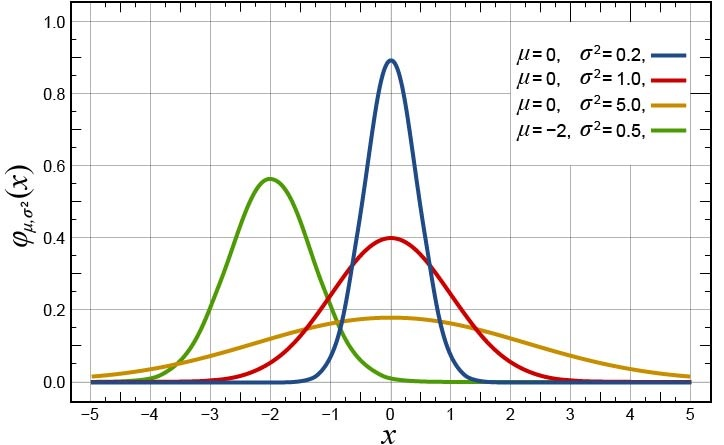
\includegraphics[width=0.8\textwidth]{Figures/Normal_Distribution_PDF.JPG}
\end{figure}

\end{frame}